\documentclass[12pt]{article}
\usepackage[english]{babel}
\usepackage[utf8x]{inputenc}
\usepackage{amsmath}
\usepackage{graphicx}
\usepackage[colorinlistoftodos]{todonotes}
\usepackage{enumerate}
\usepackage{booktabs}
\usepackage{tikz}
\usetikzlibrary{automata,positioning}
\usetikzlibrary{automata,chains}
\usetikzlibrary{arrows,automata}

\usepackage{algorithm}
\usepackage{algpseudocode}
\makeatletter
\def\BState{\State\hskip-\ALG@thistlm}
\algnewcommand{\Inputs}[1]{%
  \State \textbf{Inputs:}
  \Statex \hspace*{\algorithmicindent}\parbox[t]{.8\linewidth}{\raggedright #1}
}
\algnewcommand{\Initialize}[1]{%
  \State \textbf{Initialize:}
  \Statex \hspace*{\algorithmicindent}\parbox[t]{.8\linewidth}{\raggedright #1}
}


\begin{document}

\begin{titlepage}

\newcommand{\HRule}{\rule{\linewidth}{0.5mm}} % Defines a new command for the horizontal lines, change thickness here

\center % Center everything on the page
 
%=============================================
%	HEADING SECTIONS
\textsc{\LARGE ShanghaiTech University}\\[1.5cm] % Name of your university/college
\textsc{\Large Computer Networks}\\[0.5cm] % Major heading such as course name
\textsc{\large Spring 2016}\\[0.5cm] % Minor heading such as course title


%=============================================
%	TITLE SECTION
\HRule \\[0.4cm]
{ \huge \bfseries Project 3: Routing Algorithms via Python}\\[0.4cm] % Title of your document
\HRule \\[1.5cm]
 
 
%=============================================
%	AUTHOR SECTION
\begin{minipage}{0.4\textwidth}
\begin{flushleft} \large
\emph{Author:}\\
Xin \textsc{Gao} % Your name
\end{flushleft}
\end{minipage}
~
\begin{minipage}{0.4\textwidth}
\begin{flushright} \large
\emph{Advisor:} \\
Prof. Ziyu \textsc{Shao} % Supervisor's Name
\end{flushright}
\end{minipage}\\[2cm]

% If you don't want a supervisor, uncomment the two lines below and remove the section above
%\Large \emph{Author:}\\
%John \textsc{Smith}\\[3cm] % Your name


%=============================================
%	DATE SECTION
{\large \today}\\[2cm] % Date, change the \today to a set date if you want to be precise


%=============================================
%	LOGO SECTION
%\includegraphics{logo.png}\\[1cm] % Include a department/university logo - this will require the graphicx package


%=============================================
\vfill % Fill the rest of the page with whitespace

\end{titlepage}




%========================================================= 
% Project Description
\section{Project Description}
\textbf{Routing Algorithms via Python.} 

%========================================================= 
% Introduction
\section{Introduction}
\paragraph{} 
The goal of the project is to implement two routing algorithms (link-state routing and distance-vector routing) via Python. The input is the metro map of  Shanghai and arbitrary two stations. I use Chinese names of stations. The output is the least delay path or the least switching times with delay as low as possible. 

\paragraph{}
In my project, I use Dijkstra algorithm as the link-state routing algorithm. Link-state routing algorithm is a global routing algorithm. It uses all the information of the network to compute the least cost path between any two points. The information includes the topology of the network and all the link price. The process of Dijkstra algorithm is:

\begin{algorithm}
\caption{Dijkstra algorithm for source node $u$ (Ref: James F. Kurose, Keith W. Ross, \textit{Computer Network: A Top-Down Approach})}\label{alg1}
\begin{algorithmic}[1]
%\Inputs{$$}
\State $N=\{u\}$
\For {all nodes $v$} 
\If {$v$ is a neighbor of $u$} 
\State then $D(v)=\infty$ 
\EndIf 
\EndFor

\While{$N\neq S$}
\State find $w$ not in $N$ such that $D(w)$ is a minimum
\State add $w$ to $N$
\State update $D(v)$ for each neighbor $v$ of $w$ and not in $N$:
\State $D(v)=\min(D(v),D(w)+c(w,v)$
\EndWhile

\end{algorithmic}
\end{algorithm}



\paragraph{}
In the project, I use Bellman-Ford algorithm as the distance-vector routing algorithm. Distance-vector routing algorithm is a decentralized routing algorithm. In this algorithm, each nodes calculate path with local information at the beginning. The local information in this project is the set of links connected directly to it. In each iteration, each node will exchange information with it neighborhoods and update the information it has. After some iterations, each node will have all the information of the network and the path it compute is optimal. 

\begin{algorithm}
\caption{Bellman-Ford algorithm for source node $u$}\label{alg2}
\begin{algorithmic}[1]
%\Inputs{$$}
\For {all nodes $v$}
\If {$v\neq u$}
\State $D(v)=\infty$
\Else
\State $D(v)=0$
\EndIf
\EndFor
\State $i=1$
\For {$i\leq \left|S\right|-1$}
\For {all edge $w-v$} 
\If {$D(v)>D(w)+c(w,v)$} 
\State then $D(v)=D(w)+c(w,v)$ 
\EndIf 
\EndFor
\State $i++$
\EndFor
\end{algorithmic}
\end{algorithm}

\paragraph{}
Dijkstra algorithm is much faster than Bellman-Ford algorithm. Since Dijkstra algorithm compute the least path using global information from the beginning. In Bellman-Ford algorithm, nodes has to exchange local information with neighbors, it takes long time for convergence. However, Bellman-Ford algorithm is scalable, while Dijkstra algorithm is not. 


%========================================================= 
% Simulation Results
\section{Simulation}
\paragraph{}
In the simulation, I write the two routing algorithms according to the introduction part of the report. These two algorithms can compute the  least delay path directly. However, how to compute the least switch times path can not is a challenge. In my simulation, I refer to the solution of Zhaoxi Wu. His solution is: if there is an intersection point of several lines, number this point for different line with different number. If we want the least delay path, set the delays between these different numbered station (in fact they are the same station with different number) equal to 0. If we want the least switch time path, set the delays between these different numbered station equal to infinity. I changed Wu's solution in the following way: when compute the least delay path, it's the same as Wu's solution; however, when compute the least switch times path I set the delays equal to $1000$, which is much larger than any delay between two directly connected nodes. The result of the simulation proves that my solution is effective. Some of my simulation result are shown in figures.

\begin{figure}[H]
	\begin{center}
		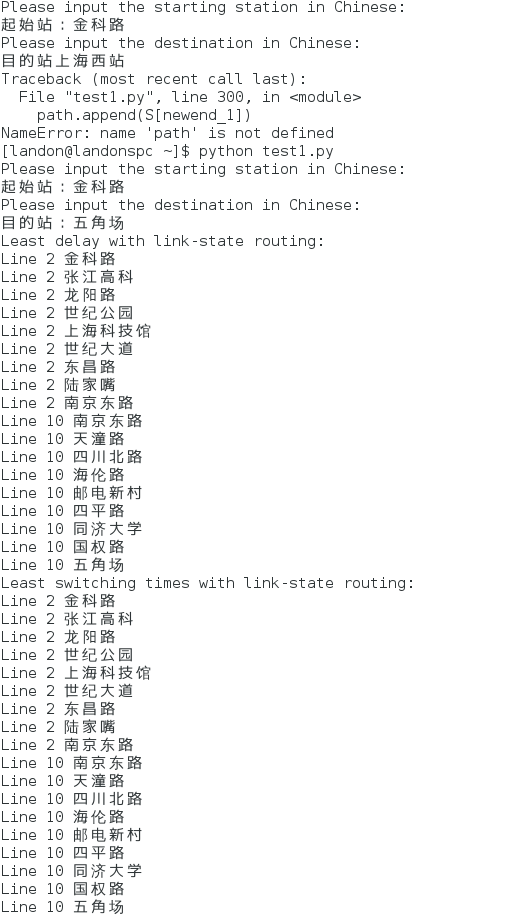
\includegraphics[width=0.8\textwidth]{figures/1}
	\end{center}
	\caption{Metro Topology}
	\label{1}
\end{figure}
\begin{figure}[H]
	\begin{center}
		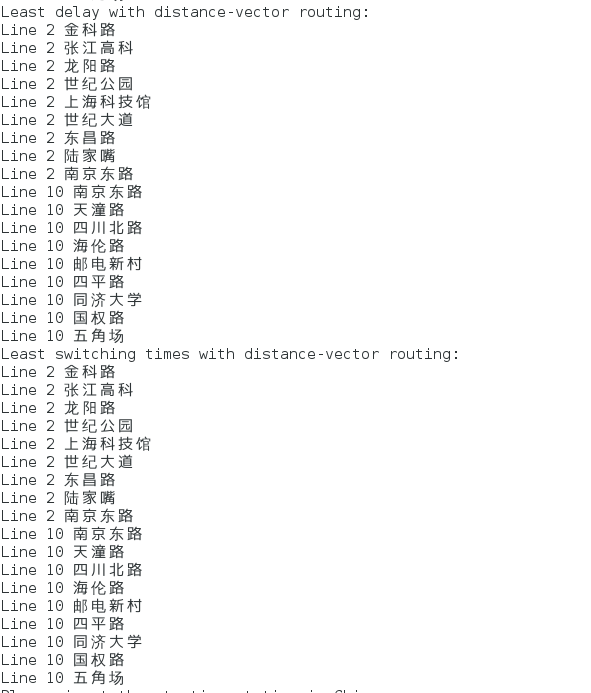
\includegraphics[width=1\textwidth]{figures/2}
	\end{center}
	\caption{Metro Topology}
	\label{1}
\end{figure}
\begin{figure}[H]
	\begin{center}
		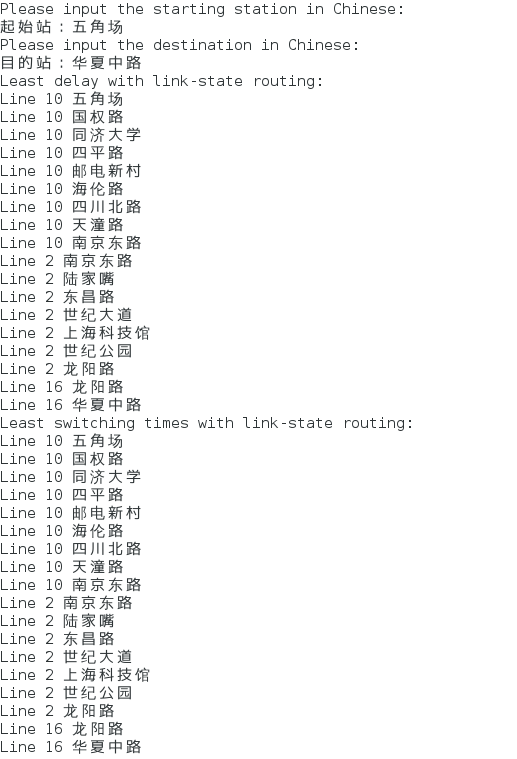
\includegraphics[width=1\textwidth]{figures/3}
	\end{center}
	\caption{Metro Topology}
	\label{1}
\end{figure}
\begin{figure}[H]
	\begin{center}
		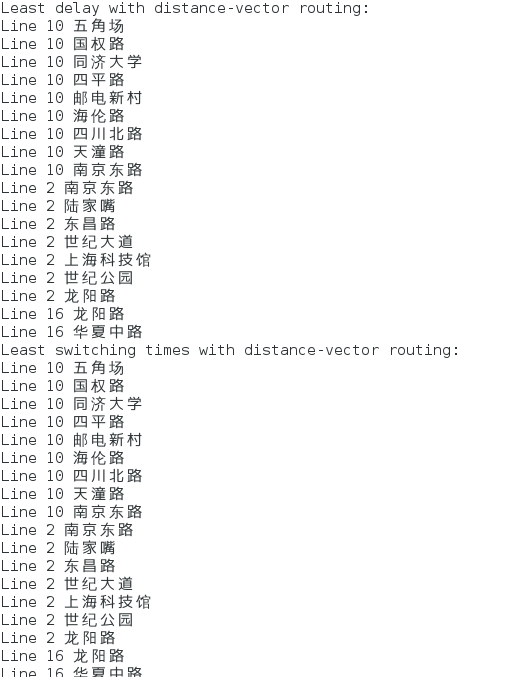
\includegraphics[width=1\textwidth]{figures/4}
	\end{center}
	\caption{Metro Topology}
	\label{1}
\end{figure}
\begin{figure}[H]
	\begin{center}
		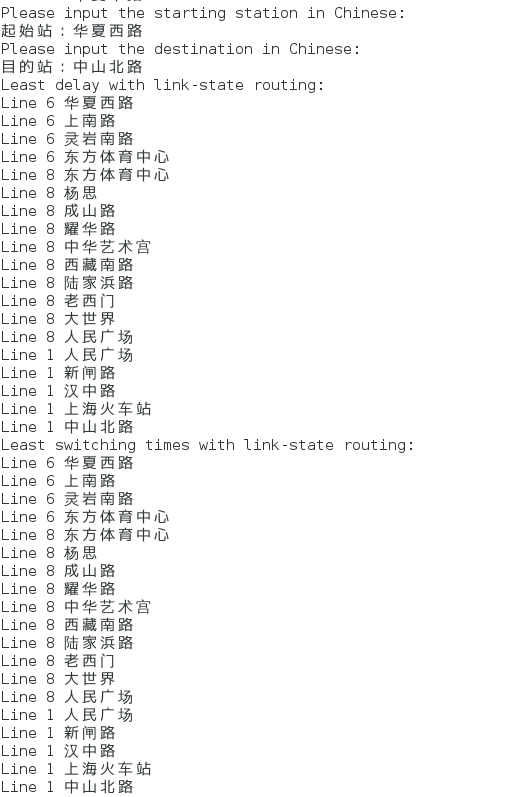
\includegraphics[width=1\textwidth]{figures/5}
	\end{center}
	\caption{Metro Topology}
	\label{1}
\end{figure}
\begin{figure}[H]
	\begin{center}
		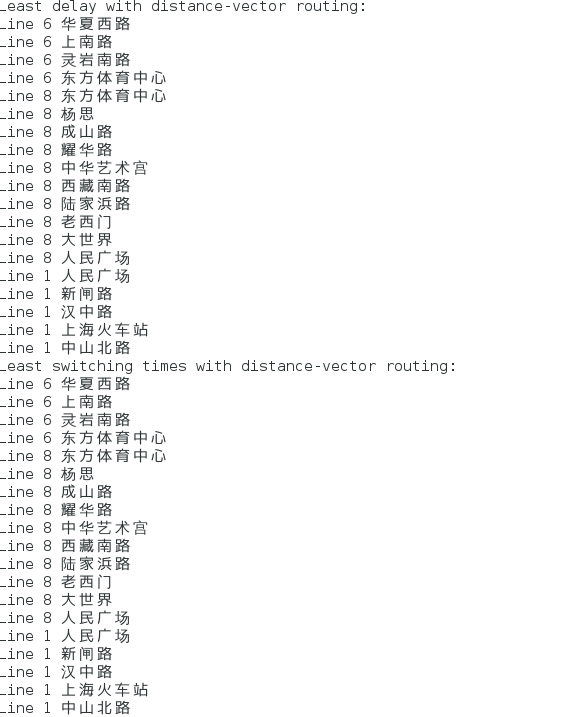
\includegraphics[width=1\textwidth]{figures/6}
	\end{center}
	\caption{Metro Topology}
	\label{1}
\end{figure}

Comparing the simulation result with path result of Gaode Map app, the two result are exactly the same. This proves that my algorithms are correct.


%========================================================= 
% Analysis of the Simulation Results & Theoretic Results
%\section{Analysis}

%---------------------------------------------------------
% Theoretic Results
%\subsection{Theoretic Results}


%---------------------------------------------------------
% Analysis
%\subsection{Results Analysis}
%\paragraph{}

\section{Conclusion}
\paragraph{}
From the project I understand further about the link-state algorithm and 
distance-vector algorithm. I realised the these two algorithms using python. To compute the least switch times path, I use a solution referred to my classmate Zhaoxi Wu. I did some change about the solution and the new solution is available. From the simulation I conclude that link-state algorithm is much faster than distance-vector algorithm since the previous one is a global algorithm while the latter one is a distributed algorithm. However, distributed algorithm is scalable, while the global algorithm is not. But in this project, the scalability of link-state algorithm is not reflected. 

\end{document}